\documentclass[1p]{elsarticle_modified}
%\bibliographystyle{elsarticle-num}

%\usepackage[colorlinks]{hyperref}
%\usepackage{abbrmath_seonhwa} %\Abb, \Ascr, \Acal ,\Abf, \Afrak
\usepackage{amsfonts}
\usepackage{amssymb}
\usepackage{amsmath}
\usepackage{amsthm}
\usepackage{scalefnt}
\usepackage{amsbsy}
\usepackage{kotex}
\usepackage{caption}
\usepackage{subfig}
\usepackage{color}
\usepackage{graphicx}
\usepackage{xcolor} %% white, black, red, green, blue, cyan, magenta, yellow
\usepackage{float}
\usepackage{setspace}
\usepackage{hyperref}

\usepackage{tikz}
\usetikzlibrary{arrows}

\usepackage{multirow}
\usepackage{array} % fixed length table
\usepackage{hhline}

%%%%%%%%%%%%%%%%%%%%%
\makeatletter
\renewcommand*\env@matrix[1][\arraystretch]{%
	\edef\arraystretch{#1}%
	\hskip -\arraycolsep
	\let\@ifnextchar\new@ifnextchar
	\array{*\c@MaxMatrixCols c}}
\makeatother %https://tex.stackexchange.com/questions/14071/how-can-i-increase-the-line-spacing-in-a-matrix
%%%%%%%%%%%%%%%

\usepackage[normalem]{ulem}

\newcommand{\msout}[1]{\ifmmode\text{\sout{\ensuremath{#1}}}\else\sout{#1}\fi}
%SOURCE: \msout is \stkout macro in https://tex.stackexchange.com/questions/20609/strikeout-in-math-mode

\newcommand{\cancel}[1]{
	\ifmmode
	{\color{red}\msout{#1}}
	\else
	{\color{red}\sout{#1}}
	\fi
}

\newcommand{\add}[1]{
	{\color{blue}\uwave{#1}}
}

\newcommand{\replace}[2]{
	\ifmmode
	{\color{red}\msout{#1}}{\color{blue}\uwave{#2}}
	\else
	{\color{red}\sout{#1}}{\color{blue}\uwave{#2}}
	\fi
}

\newcommand{\Sol}{\mathcal{S}} %segment
\newcommand{\D}{D} %diagram
\newcommand{\A}{\mathcal{A}} %arc


%%%%%%%%%%%%%%%%%%%%%%%%%%%%%5 test

\def\sl{\operatorname{\textup{SL}}(2,\Cbb)}
\def\psl{\operatorname{\textup{PSL}}(2,\Cbb)}
\def\quan{\mkern 1mu \triangleright \mkern 1mu}

\theoremstyle{definition}
\newtheorem{thm}{Theorem}[section]
\newtheorem{prop}[thm]{Proposition}
\newtheorem{lem}[thm]{Lemma}
\newtheorem{ques}[thm]{Question}
\newtheorem{cor}[thm]{Corollary}
\newtheorem{defn}[thm]{Definition}
\newtheorem{exam}[thm]{Example}
\newtheorem{rmk}[thm]{Remark}
\newtheorem{alg}[thm]{Algorithm}

\newcommand{\I}{\sqrt{-1}}
\begin{document}

%\begin{frontmatter}
%
%\title{Boundary parabolic representations of knots up to 8 crossings}
%
%%% Group authors per affiliation:
%\author{Yunhi Cho} 
%\address{Department of Mathematics, University of Seoul, Seoul, Korea}
%\ead{yhcho@uos.ac.kr}
%
%
%\author{Seonhwa Kim} %\fnref{s_kim}}
%\address{Center for Geometry and Physics, Institute for Basic Science, Pohang, 37673, Korea}
%\ead{ryeona17@ibs.re.kr}
%
%\author{Hyuk Kim}
%\address{Department of Mathematical Sciences, Seoul National University, Seoul 08826, Korea}
%\ead{hyukkim@snu.ac.kr}
%
%\author{Seokbeom Yoon}
%\address{Department of Mathematical Sciences, Seoul National University, Seoul, 08826,  Korea}
%\ead{sbyoon15@snu.ac.kr}
%
%\begin{abstract}
%We find all boundary parabolic representation of knots up to 8 crossings.
%
%\end{abstract}
%\begin{keyword}
%    \MSC[2010] 57M25 
%\end{keyword}
%
%\end{frontmatter}

%\linenumbers
%\tableofcontents
%
\newcommand\colored[1]{\textcolor{white}{\rule[-0.35ex]{0.8em}{1.4ex}}\kern-0.8em\color{red} #1}%
%\newcommand\colored[1]{\textcolor{white}{ #1}\kern-2.17ex	\textcolor{white}{ #1}\kern-1.81ex	\textcolor{white}{ #1}\kern-2.15ex\color{red}#1	}

{\Large $\underline{10_{98}~(K10a_{96})}$}

\setlength{\tabcolsep}{10pt}
\renewcommand{\arraystretch}{1.6}
\vspace{1cm}\begin{tabular}{m{100pt}>{\centering\arraybackslash}m{274pt}}
\multirow{5}{120pt}{
	\centering
	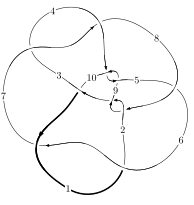
\includegraphics[width=112pt]{../../../GIT/diagram.site/diagram/png/182_10_98.png}\\
\ \ \ A knot diagram\footnotemark}&
\allowdisplaybreaks
\textbf{Linearized knot diagam} \\
\cline{2-2}
 &
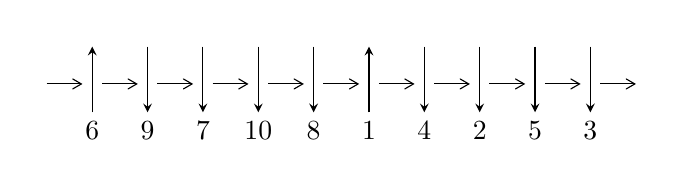
\begin{tikzpicture}[x=20pt, y=17pt]
	% nodes
	\node (C0) at (0, 0) {};
	\node (C1) at (1, 0) {};
	\node (C1U) at (1, +1) {};
	\node (C1D) at (1, -1) {6};

	\node (C2) at (2, 0) {};
	\node (C2U) at (2, +1) {};
	\node (C2D) at (2, -1) {9};

	\node (C3) at (3, 0) {};
	\node (C3U) at (3, +1) {};
	\node (C3D) at (3, -1) {7};

	\node (C4) at (4, 0) {};
	\node (C4U) at (4, +1) {};
	\node (C4D) at (4, -1) {10};

	\node (C5) at (5, 0) {};
	\node (C5U) at (5, +1) {};
	\node (C5D) at (5, -1) {8};

	\node (C6) at (6, 0) {};
	\node (C6U) at (6, +1) {};
	\node (C6D) at (6, -1) {1};

	\node (C7) at (7, 0) {};
	\node (C7U) at (7, +1) {};
	\node (C7D) at (7, -1) {4};

	\node (C8) at (8, 0) {};
	\node (C8U) at (8, +1) {};
	\node (C8D) at (8, -1) {2};

	\node (C9) at (9, 0) {};
	\node (C9U) at (9, +1) {};
	\node (C9D) at (9, -1) {5};

	\node (C10) at (10, 0) {};
	\node (C10U) at (10, +1) {};
	\node (C10D) at (10, -1) {3};
	\node (C11) at (11, 0) {};

	% arrows
	\draw[->,>={angle 60}]
	(C0) edge (C1) (C1) edge (C2) (C2) edge (C3) (C3) edge (C4) (C4) edge (C5) (C5) edge (C6) (C6) edge (C7) (C7) edge (C8) (C8) edge (C9) (C9) edge (C10) (C10) edge (C11) ;	\draw[->,>=stealth]
	(C1D) edge (C1U) (C2U) edge (C2D) (C3U) edge (C3D) (C4U) edge (C4D) (C5U) edge (C5D) (C6D) edge (C6U) (C7U) edge (C7D) (C8U) edge (C8D) (C9U) edge (C9D) (C10U) edge (C10D) ;
	\end{tikzpicture} \\
\hhline{~~} \\& 
\textbf{Solving Sequence} \\ \cline{2-2} 
 &
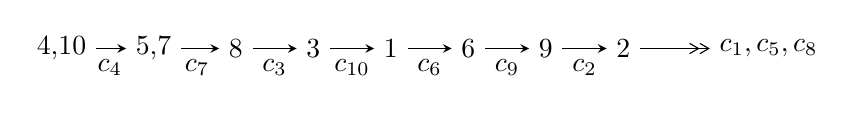
\begin{tikzpicture}[x=28pt, y=7pt]
	% node
	\node (A0) at (-1/8, 0) {4,10};
	\node (A1) at (17/16, 0) {5,7};
	\node (A2) at (17/8, 0) {8};
	\node (A3) at (25/8, 0) {3};
	\node (A4) at (33/8, 0) {1};
	\node (A5) at (41/8, 0) {6};
	\node (A6) at (49/8, 0) {9};
	\node (A7) at (57/8, 0) {2};
	\node (C1) at (1/2, -1) {$c_{4}$};
	\node (C2) at (13/8, -1) {$c_{7}$};
	\node (C3) at (21/8, -1) {$c_{3}$};
	\node (C4) at (29/8, -1) {$c_{10}$};
	\node (C5) at (37/8, -1) {$c_{6}$};
	\node (C6) at (45/8, -1) {$c_{9}$};
	\node (C7) at (53/8, -1) {$c_{2}$};
	\node (A8) at (9, 0) {$c_{1},c_{5},c_{8}$};

	% edge
	\draw[->,>=stealth]	
	(A0) edge (A1) (A1) edge (A2) (A2) edge (A3) (A3) edge (A4) (A4) edge (A5) (A5) edge (A6) (A6) edge (A7) ;
	\draw[->>,>={angle 60}]	
	(A7) edge (A8);
\end{tikzpicture} \\ 

\end{tabular} \\

\footnotetext{
The image of knot diagram is generated by the software ``\textbf{Draw programme}" developed by Andrew Bartholomew(\url{http://www.layer8.co.uk/maths/draw/index.htm\#Running-draw}), where we modified some parts for our purpose(\url{https://github.com/CATsTAILs/LinksPainter}).
}\phantom \\ \newline 
\centering \textbf{Ideals for irreducible components\footnotemark of $X_{\text{par}}$} 
 
\begin{align*}
I^u_{1}&=\langle 
-4789953 u^{11}+15314376 u^{10}+\cdots+9342488 b+9873021,\\
\phantom{I^u_{1}}&\phantom{= \langle  }-16446192 u^{11}+38491161 u^{10}+\cdots+23356220 a+2924955,\\
\phantom{I^u_{1}}&\phantom{= \langle  }3 u^{12}-9 u^{11}+22 u^{10}-42 u^9+70 u^8-110 u^7+139 u^6-157 u^5+149 u^4-106 u^3+64 u^2-20 u+5\rangle \\
I^u_{2}&=\langle 
- u^9- u^8-3 u^7-3 u^6-5 u^5-5 u^4- u^2 a-4 u^3-4 u^2+b- a-3 u-2,\;6 u^9 a-3 u^9+\cdots+6 a-7,\\
\phantom{I^u_{2}}&\phantom{= \langle  }u^{10}+u^9+3 u^8+3 u^7+5 u^6+5 u^5+4 u^4+4 u^3+3 u^2+2 u+1\rangle \\
I^u_{3}&=\langle 
b+u,\;2 a- u-1,\;u^2+1\rangle \\
I^u_{4}&=\langle 
b,\;a-1,\;u^3+u-1\rangle \\
I^u_{5}&=\langle 
b-1,\;a- u-1,\;u^3+u-1\rangle \\
I^u_{6}&=\langle 
b-1,\;u^3 a- u^3+a u-2 u-1\rangle \\
\\
\end{align*}
\raggedright * 5 irreducible components of $\dim_{\mathbb{C}}=0$, with total 40 representations.\\
\raggedright * 1 irreducible components of $\dim_{\mathbb{C}}=1$ \\
\footnotetext{All coefficients of polynomials are rational numbers. But the coefficients are sometimes approximated in decimal forms when there is not enough margin.}
\newpage
\renewcommand{\arraystretch}{1}
\centering \section*{I. $I^u_{1}= \langle -4.79\times10^{6} u^{11}+1.53\times10^{7} u^{10}+\cdots+9.34\times10^{6} b+9.87\times10^{6},\;-1.64\times10^{7} u^{11}+3.85\times10^{7} u^{10}+\cdots+2.34\times10^{7} a+2.92\times10^{6},\;3 u^{12}-9 u^{11}+\cdots-20 u+5 \rangle$}
\flushleft \textbf{(i) Arc colorings}\\
\begin{tabular}{m{7pt} m{180pt} m{7pt} m{180pt} }
\flushright $a_{4}=$&$\begin{pmatrix}1\\0\end{pmatrix}$ \\
\flushright $a_{10}=$&$\begin{pmatrix}0\\u\end{pmatrix}$ \\
\flushright $a_{5}=$&$\begin{pmatrix}1\\u^2\end{pmatrix}$ \\
\flushright $a_{7}=$&$\begin{pmatrix}0.704146 u^{11}-1.64800 u^{10}+\cdots+5.67136 u-0.125232\\0.512706 u^{11}-1.63922 u^{10}+\cdots+5.56042 u-1.05679\end{pmatrix}$ \\
\flushright $a_{8}=$&$\begin{pmatrix}0.191440 u^{11}-0.00878657 u^{10}+\cdots+0.110936 u+0.931555\\0.512706 u^{11}-1.63922 u^{10}+\cdots+5.56042 u-1.05679\end{pmatrix}$ \\
\flushright $a_{3}=$&$\begin{pmatrix}0.0685395 u^{11}-0.0742645 u^{10}+\cdots-2.54876 u+1.65234\\-0.524747 u^{11}+1.36714 u^{10}+\cdots-1.44636 u+0.100143\end{pmatrix}$ \\
\flushright $a_{1}=$&$\begin{pmatrix}-0.159552 u^{11}+0.582496 u^{10}+\cdots-1.27370 u-0.346141\\0.514632 u^{11}-1.19725 u^{10}+\cdots+3.19361 u-0.462234\end{pmatrix}$ \\
\flushright $a_{6}=$&$\begin{pmatrix}0.173499 u^{11}-0.281506 u^{10}+\cdots+1.01679 u+1.07875\\0.0278643 u^{11}-0.396636 u^{10}+\cdots+2.71393 u-0.664239\end{pmatrix}$ \\
\flushright $a_{9}=$&$\begin{pmatrix}u\\u^3+u\end{pmatrix}$ \\
\flushright $a_{2}=$&$\begin{pmatrix}0.169639 u^{11}-0.151768 u^{10}+\cdots-4.91002 u+2.50685\\-0.477984 u^{11}+1.17054 u^{10}+\cdots-2.47082 u+0.578331\end{pmatrix}$\\&\end{tabular}
\flushleft \textbf{(ii) Obstruction class $= -1$}\\~\\
\flushleft \textbf{(iii) Cusp Shapes $= \frac{4958289}{2335622} u^{11}-\frac{5676297}{1167811} u^{10}+\cdots+\frac{80416785}{2335622} u-\frac{35331855}{2335622}$}\\~\\
\newpage\renewcommand{\arraystretch}{1}
\flushleft \textbf{(iv) u-Polynomials at the component}\newline \\
\begin{tabular}{m{50pt}|m{274pt}}
Crossings & \hspace{64pt}u-Polynomials at each crossing \\
\hline $$\begin{aligned}c_{1},c_{6}\end{aligned}$$&$\begin{aligned}
&3(3 u^{12}+9 u^{11}+\cdots+26 u+5)
\end{aligned}$\\
\hline $$\begin{aligned}c_{2},c_{3},c_{7}\\c_{8}\end{aligned}$$&$\begin{aligned}
&u^{12}-2 u^{11}+u^9+3 u^7+u^6-15 u^5+21 u^4-14 u^3+3 u^2+u+2
\end{aligned}$\\
\hline $$\begin{aligned}c_{4},c_{9}\end{aligned}$$&$\begin{aligned}
&3(3 u^{12}+9 u^{11}+\cdots+20 u+5)
\end{aligned}$\\
\hline $$\begin{aligned}c_{5},c_{10}\end{aligned}$$&$\begin{aligned}
&2(2 u^{12}-4 u^{11}+\cdots+12 u+3)
\end{aligned}$\\
\hline
\end{tabular}\\~\\
\newpage\renewcommand{\arraystretch}{1}
\flushleft \textbf{(v) Riley Polynomials at the component}\newline \\
\begin{tabular}{m{50pt}|m{274pt}}
Crossings & \hspace{64pt}Riley Polynomials at each crossing \\
\hline $$\begin{aligned}c_{1},c_{6}\end{aligned}$$&$\begin{aligned}
&9(9 y^{12}+87 y^{11}+\cdots-16 y+25)
\end{aligned}$\\
\hline $$\begin{aligned}c_{2},c_{3},c_{7}\\c_{8}\end{aligned}$$&$\begin{aligned}
&y^{12}-4 y^{11}+\cdots+11 y+4
\end{aligned}$\\
\hline $$\begin{aligned}c_{4},c_{9}\end{aligned}$$&$\begin{aligned}
&9(9 y^{12}+51 y^{11}+\cdots+240 y+25)
\end{aligned}$\\
\hline $$\begin{aligned}c_{5},c_{10}\end{aligned}$$&$\begin{aligned}
&4(4 y^{12}-20 y^{11}+\cdots-30 y+9)
\end{aligned}$\\
\hline
\end{tabular}\\~\\
\newpage\flushleft \textbf{(vi) Complex Volumes and Cusp Shapes}
$$\begin{array}{c|c|c}  
\text{Solutions to }I^u_{1}& \I (\text{vol} + \sqrt{-1}CS) & \text{Cusp shape}\\
 \hline 
\begin{aligned}
u &= \phantom{-}0.294163 + 0.893263 I \\
a &= -0.392558 + 0.428484 I \\
b &= \phantom{-}0.312276 - 1.374800 I\end{aligned}
 & \phantom{-}0.93953 - 1.28267 I & -9.97159 + 5.49540 I \\ \hline\begin{aligned}
u &= \phantom{-}0.294163 - 0.893263 I \\
a &= -0.392558 - 0.428484 I \\
b &= \phantom{-}0.312276 + 1.374800 I\end{aligned}
 & \phantom{-}0.93953 + 1.28267 I & -9.97159 - 5.49540 I \\ \hline\begin{aligned}
u &= -0.132310 + 1.149860 I \\
a &= -0.019852 + 0.332765 I \\
b &= -0.435810 - 0.817904 I\end{aligned}
 & \phantom{-}3.72744 - 0.65506 I & \phantom{-}0.96539 + 2.36054 I \\ \hline\begin{aligned}
u &= -0.132310 - 1.149860 I \\
a &= -0.019852 - 0.332765 I \\
b &= -0.435810 + 0.817904 I\end{aligned}
 & \phantom{-}3.72744 + 0.65506 I & \phantom{-}0.96539 - 2.36054 I \\ \hline\begin{aligned}
u &= \phantom{-}1.258330 + 0.213822 I \\
a &= -1.45041 + 0.16116 I \\
b &= -1.325110 + 0.371579 I\end{aligned}
 & -10.52620 + 7.73722 I & -13.2705 - 5.1580 I \\ \hline\begin{aligned}
u &= \phantom{-}1.258330 - 0.213822 I \\
a &= -1.45041 - 0.16116 I \\
b &= -1.325110 - 0.371579 I\end{aligned}
 & -10.52620 - 7.73722 I & -13.2705 + 5.1580 I \\ \hline\begin{aligned}
u &= -0.77981 + 1.24219 I \\
a &= -1.28771 - 0.68411 I \\
b &= -1.170890 + 0.448059 I\end{aligned}
 & -1.38664 + 8.65525 I & -8.05360 - 7.75821 I \\ \hline\begin{aligned}
u &= -0.77981 - 1.24219 I \\
a &= -1.28771 + 0.68411 I \\
b &= -1.170890 - 0.448059 I\end{aligned}
 & -1.38664 - 8.65525 I & -8.05360 + 7.75821 I \\ \hline\begin{aligned}
u &= \phantom{-}0.66776 + 1.32565 I \\
a &= \phantom{-}1.16439 - 0.95583 I \\
b &= \phantom{-}1.36378 + 0.57208 I\end{aligned}
 & -7.0244 - 14.4129 I & -10.01184 + 7.82077 I \\ \hline\begin{aligned}
u &= \phantom{-}0.66776 - 1.32565 I \\
a &= \phantom{-}1.16439 + 0.95583 I \\
b &= \phantom{-}1.36378 - 0.57208 I\end{aligned}
 & -7.0244 + 14.4129 I & -10.01184 - 7.82077 I\\
 \hline 
 \end{array}$$\newpage$$\begin{array}{c|c|c}  
\text{Solutions to }I^u_{1}& \I (\text{vol} + \sqrt{-1}CS) & \text{Cusp shape}\\
 \hline 
\begin{aligned}
u &= \phantom{-}0.191864 + 0.381263 I \\
a &= \phantom{-}0.986139 + 0.917994 I \\
b &= \phantom{-}0.255755 + 0.338417 I\end{aligned}
 & -0.534161 - 1.008590 I & -7.65789 + 6.71362 I \\ \hline\begin{aligned}
u &= \phantom{-}0.191864 - 0.381263 I \\
a &= \phantom{-}0.986139 - 0.917994 I \\
b &= \phantom{-}0.255755 - 0.338417 I\end{aligned}
 & -0.534161 + 1.008590 I & -7.65789 - 6.71362 I\\
 \hline 
 \end{array}$$\newpage\newpage\renewcommand{\arraystretch}{1}
\centering \section*{II. $I^u_{2}= \langle - u^9- u^8+\cdots- a-2,\;6 u^9 a-3 u^9+\cdots+6 a-7,\;u^{10}+u^9+\cdots+2 u+1 \rangle$}
\flushleft \textbf{(i) Arc colorings}\\
\begin{tabular}{m{7pt} m{180pt} m{7pt} m{180pt} }
\flushright $a_{4}=$&$\begin{pmatrix}1\\0\end{pmatrix}$ \\
\flushright $a_{10}=$&$\begin{pmatrix}0\\u\end{pmatrix}$ \\
\flushright $a_{5}=$&$\begin{pmatrix}1\\u^2\end{pmatrix}$ \\
\flushright $a_{7}=$&$\begin{pmatrix}a\\u^9+u^8+3 u^7+3 u^6+5 u^5+5 u^4+u^2 a+4 u^3+4 u^2+a+3 u+2\end{pmatrix}$ \\
\flushright $a_{8}=$&$\begin{pmatrix}- u^9- u^8-3 u^7-3 u^6-5 u^5-5 u^4- u^2 a-4 u^3-4 u^2-3 u-2\\u^9+u^8+3 u^7+3 u^6+5 u^5+5 u^4+u^2 a+4 u^3+4 u^2+a+3 u+2\end{pmatrix}$ \\
\flushright $a_{3}=$&$\begin{pmatrix}u^9 a+u^9+\cdots+2 a- u\\- u^5 a+u^6-2 u^3 a+2 u^4- a u+2 u^2\end{pmatrix}$ \\
\flushright $a_{1}=$&$\begin{pmatrix}- u^9 a-\frac{1}{2} u^9+\cdots-2 a+\frac{5}{2}\\- u^9 a-2 u^9+\cdots-2 a-1\end{pmatrix}$ \\
\flushright $a_{6}=$&$\begin{pmatrix}-2 u^9 a-\frac{1}{2} u^9+\cdots- a+\frac{1}{2}\\u^9+u^8+\cdots+3 u+2\end{pmatrix}$ \\
\flushright $a_{9}=$&$\begin{pmatrix}u\\u^3+u\end{pmatrix}$ \\
\flushright $a_{2}=$&$\begin{pmatrix}u^9 a+u^9+\cdots+2 a-1\\-1\end{pmatrix}$\\&\end{tabular}
\flushleft \textbf{(ii) Obstruction class $= -1$}\\~\\
\flushleft \textbf{(iii) Cusp Shapes $= -4 u^9-4 u^8-8 u^7-8 u^6-8 u^5-12 u^4-4 u^2-4 u-10$}\\~\\
\newpage\renewcommand{\arraystretch}{1}
\flushleft \textbf{(iv) u-Polynomials at the component}\newline \\
\begin{tabular}{m{50pt}|m{274pt}}
Crossings & \hspace{64pt}u-Polynomials at each crossing \\
\hline $$\begin{aligned}c_{1},c_{6}\end{aligned}$$&$\begin{aligned}
&(u^{10}- u^9+5 u^8-5 u^7+9 u^6-9 u^5+6 u^4-6 u^3+u^2+1)^2
\end{aligned}$\\
\hline $$\begin{aligned}c_{2},c_{3},c_{7}\\c_{8}\end{aligned}$$&$\begin{aligned}
&u^{20}-2 u^{19}+\cdots-58 u+31
\end{aligned}$\\
\hline $$\begin{aligned}c_{4},c_{9}\end{aligned}$$&$\begin{aligned}
&(u^{10}- u^9+3 u^8-3 u^7+5 u^6-5 u^5+4 u^4-4 u^3+3 u^2-2 u+1)^2
\end{aligned}$\\
\hline $$\begin{aligned}c_{5},c_{10}\end{aligned}$$&$\begin{aligned}
&2(2 u^{20}-13 u^{18}+\cdots-518 u+121)
\end{aligned}$\\
\hline
\end{tabular}\\~\\
\newpage\renewcommand{\arraystretch}{1}
\flushleft \textbf{(v) Riley Polynomials at the component}\newline \\
\begin{tabular}{m{50pt}|m{274pt}}
Crossings & \hspace{64pt}Riley Polynomials at each crossing \\
\hline $$\begin{aligned}c_{1},c_{6}\end{aligned}$$&$\begin{aligned}
&(y^{10}+9 y^9+33 y^8+59 y^7+41 y^6-21 y^5-44 y^4-6 y^3+13 y^2+2 y+1)^{2}
\end{aligned}$\\
\hline $$\begin{aligned}c_{2},c_{3},c_{7}\\c_{8}\end{aligned}$$&$\begin{aligned}
&y^{20}-14 y^{19}+\cdots-388 y+961
\end{aligned}$\\
\hline $$\begin{aligned}c_{4},c_{9}\end{aligned}$$&$\begin{aligned}
&(y^{10}+5 y^9+13 y^8+19 y^7+17 y^6+7 y^5-2 y^3+y^2+2 y+1)^2
\end{aligned}$\\
\hline $$\begin{aligned}c_{5},c_{10}\end{aligned}$$&$\begin{aligned}
&4(4 y^{20}-52 y^{19}+\cdots-56574 y+14641)
\end{aligned}$\\
\hline
\end{tabular}\\~\\
\newpage\flushleft \textbf{(vi) Complex Volumes and Cusp Shapes}
$$\begin{array}{c|c|c}  
\text{Solutions to }I^u_{2}& \I (\text{vol} + \sqrt{-1}CS) & \text{Cusp shape}\\
 \hline 
\begin{aligned}
u &= \phantom{-}0.584958 + 0.771492 I \\
a &= -0.759755 + 0.346084 I \\
b &= -1.50393 + 0.39581 I\end{aligned}
 & -8.22706 - 2.31006 I & -12.86369 + 3.52133 I \\ \hline\begin{aligned}
u &= \phantom{-}0.584958 + 0.771492 I \\
a &= \phantom{-}0.94152 - 1.29105 I \\
b &= \phantom{-}1.24454 + 0.70845 I\end{aligned}
 & -8.22706 - 2.31006 I & -12.86369 + 3.52133 I \\ \hline\begin{aligned}
u &= \phantom{-}0.584958 - 0.771492 I \\
a &= -0.759755 - 0.346084 I \\
b &= -1.50393 - 0.39581 I\end{aligned}
 & -8.22706 + 2.31006 I & -12.86369 - 3.52133 I \\ \hline\begin{aligned}
u &= \phantom{-}0.584958 - 0.771492 I \\
a &= \phantom{-}0.94152 + 1.29105 I \\
b &= \phantom{-}1.24454 - 0.70845 I\end{aligned}
 & -8.22706 + 2.31006 I & -12.86369 - 3.52133 I \\ \hline\begin{aligned}
u &= -0.248527 + 0.782547 I \\
a &= \phantom{-}2.10247 - 0.40028 I \\
b &= \phantom{-}1.157780 + 0.163121 I\end{aligned}
 & -2.84181 + 1.23169 I & -7.09823 - 5.44908 I \\ \hline\begin{aligned}
u &= -0.248527 + 0.782547 I \\
a &= -0.73260 - 2.58251 I \\
b &= -0.965077 + 0.285214 I\end{aligned}
 & -2.84181 + 1.23169 I & -7.09823 - 5.44908 I \\ \hline\begin{aligned}
u &= -0.248527 - 0.782547 I \\
a &= \phantom{-}2.10247 + 0.40028 I \\
b &= \phantom{-}1.157780 - 0.163121 I\end{aligned}
 & -2.84181 - 1.23169 I & -7.09823 + 5.44908 I \\ \hline\begin{aligned}
u &= -0.248527 - 0.782547 I \\
a &= -0.73260 + 2.58251 I \\
b &= -0.965077 - 0.285214 I\end{aligned}
 & -2.84181 - 1.23169 I & -7.09823 + 5.44908 I \\ \hline\begin{aligned}
u &= -0.761643 + 0.208049 I \\
a &= -0.670419 + 0.201639 I \\
b &= \phantom{-}0.255380 + 0.856092 I\end{aligned}
 & -5.70347 - 3.47839 I & -11.19503 + 2.79515 I \\ \hline\begin{aligned}
u &= -0.761643 + 0.208049 I \\
a &= -1.53048 - 0.72472 I \\
b &= -1.359950 - 0.294980 I\end{aligned}
 & -5.70347 - 3.47839 I & -11.19503 + 2.79515 I\\
 \hline 
 \end{array}$$\newpage$$\begin{array}{c|c|c}  
\text{Solutions to }I^u_{2}& \I (\text{vol} + \sqrt{-1}CS) & \text{Cusp shape}\\
 \hline 
\begin{aligned}
u &= -0.761643 - 0.208049 I \\
a &= -0.670419 - 0.201639 I \\
b &= \phantom{-}0.255380 - 0.856092 I\end{aligned}
 & -5.70347 + 3.47839 I & -11.19503 - 2.79515 I \\ \hline\begin{aligned}
u &= -0.761643 - 0.208049 I \\
a &= -1.53048 + 0.72472 I \\
b &= -1.359950 + 0.294980 I\end{aligned}
 & -5.70347 + 3.47839 I & -11.19503 - 2.79515 I \\ \hline\begin{aligned}
u &= \phantom{-}0.449566 + 1.164790 I \\
a &= -1.032640 + 0.923920 I \\
b &= -1.096360 - 0.477116 I\end{aligned}
 & \phantom{-}1.58679 - 4.14585 I & -3.01866 + 3.97600 I \\ \hline\begin{aligned}
u &= \phantom{-}0.449566 + 1.164790 I \\
a &= \phantom{-}0.0061280 - 0.0919696 I \\
b &= -0.193027 + 0.767853 I\end{aligned}
 & \phantom{-}1.58679 - 4.14585 I & -3.01866 + 3.97600 I \\ \hline\begin{aligned}
u &= \phantom{-}0.449566 - 1.164790 I \\
a &= -1.032640 - 0.923920 I \\
b &= -1.096360 + 0.477116 I\end{aligned}
 & \phantom{-}1.58679 + 4.14585 I & -3.01866 - 3.97600 I \\ \hline\begin{aligned}
u &= \phantom{-}0.449566 - 1.164790 I \\
a &= \phantom{-}0.0061280 + 0.0919696 I \\
b &= -0.193027 - 0.767853 I\end{aligned}
 & \phantom{-}1.58679 + 4.14585 I & -3.01866 - 3.97600 I \\ \hline\begin{aligned}
u &= -0.524355 + 1.163410 I \\
a &= \phantom{-}1.040500 + 0.946543 I \\
b &= \phantom{-}1.39510 - 0.62944 I\end{aligned}
 & -2.90872 + 8.28632 I & -7.82440 - 6.14881 I \\ \hline\begin{aligned}
u &= -0.524355 + 1.163410 I \\
a &= -0.364738 - 0.233686 I \\
b &= \phantom{-}0.065535 + 1.177790 I\end{aligned}
 & -2.90872 + 8.28632 I & -7.82440 - 6.14881 I \\ \hline\begin{aligned}
u &= -0.524355 - 1.163410 I \\
a &= \phantom{-}1.040500 - 0.946543 I \\
b &= \phantom{-}1.39510 + 0.62944 I\end{aligned}
 & -2.90872 - 8.28632 I & -7.82440 + 6.14881 I \\ \hline\begin{aligned}
u &= -0.524355 - 1.163410 I \\
a &= -0.364738 + 0.233686 I \\
b &= \phantom{-}0.065535 - 1.177790 I\end{aligned}
 & -2.90872 - 8.28632 I & -7.82440 + 6.14881 I\\
 \hline 
 \end{array}$$\newpage\newpage\renewcommand{\arraystretch}{1}
\centering \section*{III. $I^u_{3}= \langle b+u,\;2 a- u-1,\;u^2+1 \rangle$}
\flushleft \textbf{(i) Arc colorings}\\
\begin{tabular}{m{7pt} m{180pt} m{7pt} m{180pt} }
\flushright $a_{4}=$&$\begin{pmatrix}1\\0\end{pmatrix}$ \\
\flushright $a_{10}=$&$\begin{pmatrix}0\\u\end{pmatrix}$ \\
\flushright $a_{5}=$&$\begin{pmatrix}1\\-1\end{pmatrix}$ \\
\flushright $a_{7}=$&$\begin{pmatrix}\frac{1}{2} u+\frac{1}{2}\\- u\end{pmatrix}$ \\
\flushright $a_{8}=$&$\begin{pmatrix}\frac{3}{2} u+\frac{1}{2}\\- u\end{pmatrix}$ \\
\flushright $a_{3}=$&$\begin{pmatrix}\frac{1}{2} u+\frac{1}{2}\\1\end{pmatrix}$ \\
\flushright $a_{1}=$&$\begin{pmatrix}0.5\\\frac{1}{2} u+\frac{1}{2}\end{pmatrix}$ \\
\flushright $a_{6}=$&$\begin{pmatrix}u+\frac{1}{2}\\-\frac{1}{2} u-\frac{1}{2}\end{pmatrix}$ \\
\flushright $a_{9}=$&$\begin{pmatrix}u\\0\end{pmatrix}$ \\
\flushright $a_{2}=$&$\begin{pmatrix}\frac{1}{2} u-\frac{1}{2}\\1\end{pmatrix}$\\&\end{tabular}
\flushleft \textbf{(ii) Obstruction class $= 1$}\\~\\
\flushleft \textbf{(iii) Cusp Shapes $= -4$}\\~\\
\newpage\renewcommand{\arraystretch}{1}
\flushleft \textbf{(iv) u-Polynomials at the component}\newline \\
\begin{tabular}{m{50pt}|m{274pt}}
Crossings & \hspace{64pt}u-Polynomials at each crossing \\
\hline $$\begin{aligned}c_{1},c_{2},c_{3}\\c_{4},c_{6},c_{7}\\c_{8},c_{9}\end{aligned}$$&$\begin{aligned}
&u^2+1
\end{aligned}$\\
\hline $$\begin{aligned}c_{5},c_{10}\end{aligned}$$&$\begin{aligned}
&2(2 u^2-2 u+1)
\end{aligned}$\\
\hline
\end{tabular}\\~\\
\newpage\renewcommand{\arraystretch}{1}
\flushleft \textbf{(v) Riley Polynomials at the component}\newline \\
\begin{tabular}{m{50pt}|m{274pt}}
Crossings & \hspace{64pt}Riley Polynomials at each crossing \\
\hline $$\begin{aligned}c_{1},c_{2},c_{3}\\c_{4},c_{6},c_{7}\\c_{8},c_{9}\end{aligned}$$&$\begin{aligned}
&(y+1)^2
\end{aligned}$\\
\hline $$\begin{aligned}c_{5},c_{10}\end{aligned}$$&$\begin{aligned}
&4(4 y^2+1)
\end{aligned}$\\
\hline
\end{tabular}\\~\\
\newpage\flushleft \textbf{(vi) Complex Volumes and Cusp Shapes}
$$\begin{array}{c|c|c}  
\text{Solutions to }I^u_{3}& \I (\text{vol} + \sqrt{-1}CS) & \text{Cusp shape}\\
 \hline 
\begin{aligned}
u &= \phantom{-0.000000 -}1.000000 I \\
a &= \phantom{-}0.500000 + 0.500000 I \\
b &= \phantom{-0.000000 } -1.000000 I\end{aligned}
 & \phantom{-}1.64493\phantom{ +0.000000I} & -4.00000\phantom{ +0.000000I} \\ \hline\begin{aligned}
u &= \phantom{-0.000000 } -1.000000 I \\
a &= \phantom{-}0.500000 - 0.500000 I \\
b &= \phantom{-0.000000 -}1.000000 I\end{aligned}
 & \phantom{-}1.64493\phantom{ +0.000000I} & -4.00000\phantom{ +0.000000I}\\
 \hline 
 \end{array}$$\newpage\newpage\renewcommand{\arraystretch}{1}
\centering \section*{IV. $I^u_{4}= \langle b,\;a-1,\;u^3+u-1 \rangle$}
\flushleft \textbf{(i) Arc colorings}\\
\begin{tabular}{m{7pt} m{180pt} m{7pt} m{180pt} }
\flushright $a_{4}=$&$\begin{pmatrix}1\\0\end{pmatrix}$ \\
\flushright $a_{10}=$&$\begin{pmatrix}0\\u\end{pmatrix}$ \\
\flushright $a_{5}=$&$\begin{pmatrix}1\\u^2\end{pmatrix}$ \\
\flushright $a_{7}=$&$\begin{pmatrix}1\\0\end{pmatrix}$ \\
\flushright $a_{8}=$&$\begin{pmatrix}1\\0\end{pmatrix}$ \\
\flushright $a_{3}=$&$\begin{pmatrix}1\\0\end{pmatrix}$ \\
\flushright $a_{1}=$&$\begin{pmatrix}- u\\u\end{pmatrix}$ \\
\flushright $a_{6}=$&$\begin{pmatrix}- u^2+1\\u^2\end{pmatrix}$ \\
\flushright $a_{9}=$&$\begin{pmatrix}u\\1\end{pmatrix}$ \\
\flushright $a_{2}=$&$\begin{pmatrix}- u+1\\-1\end{pmatrix}$\\&\end{tabular}
\flushleft \textbf{(ii) Obstruction class $= -1$}\\~\\
\flushleft \textbf{(iii) Cusp Shapes $= -6$}\\~\\
\newpage\renewcommand{\arraystretch}{1}
\flushleft \textbf{(iv) u-Polynomials at the component}\newline \\
\begin{tabular}{m{50pt}|m{274pt}}
Crossings & \hspace{64pt}u-Polynomials at each crossing \\
\hline $$\begin{aligned}c_{1},c_{4},c_{6}\\c_{9},c_{10}\end{aligned}$$&$\begin{aligned}
&u^3+u+1
\end{aligned}$\\
\hline $$\begin{aligned}c_{2},c_{8}\end{aligned}$$&$\begin{aligned}
&(u+1)^3
\end{aligned}$\\
\hline $$\begin{aligned}c_{3},c_{7}\end{aligned}$$&$\begin{aligned}
&u^3
\end{aligned}$\\
\hline $$\begin{aligned}c_{5}\end{aligned}$$&$\begin{aligned}
&u^3+2 u^2+u-1
\end{aligned}$\\
\hline
\end{tabular}\\~\\
\newpage\renewcommand{\arraystretch}{1}
\flushleft \textbf{(v) Riley Polynomials at the component}\newline \\
\begin{tabular}{m{50pt}|m{274pt}}
Crossings & \hspace{64pt}Riley Polynomials at each crossing \\
\hline $$\begin{aligned}c_{1},c_{4},c_{6}\\c_{9},c_{10}\end{aligned}$$&$\begin{aligned}
&y^3+2 y^2+y-1
\end{aligned}$\\
\hline $$\begin{aligned}c_{2},c_{8}\end{aligned}$$&$\begin{aligned}
&(y-1)^3
\end{aligned}$\\
\hline $$\begin{aligned}c_{3},c_{7}\end{aligned}$$&$\begin{aligned}
&y^3
\end{aligned}$\\
\hline $$\begin{aligned}c_{5}\end{aligned}$$&$\begin{aligned}
&y^3-2 y^2+5 y-1
\end{aligned}$\\
\hline
\end{tabular}\\~\\
\newpage\flushleft \textbf{(vi) Complex Volumes and Cusp Shapes}
$$\begin{array}{c|c|c}  
\text{Solutions to }I^u_{4}& \I (\text{vol} + \sqrt{-1}CS) & \text{Cusp shape}\\
 \hline 
\begin{aligned}
u &= -0.341164 + 1.161540 I \\
a &= \phantom{-}1.00000\phantom{ +0.000000I} \\
b &= \phantom{-0.000000 } 0\end{aligned}
 & -1.64493\phantom{ +0.000000I} & -6.00000\phantom{ +0.000000I} \\ \hline\begin{aligned}
u &= -0.341164 - 1.161540 I \\
a &= \phantom{-}1.00000\phantom{ +0.000000I} \\
b &= \phantom{-0.000000 } 0\end{aligned}
 & -1.64493\phantom{ +0.000000I} & -6.00000\phantom{ +0.000000I} \\ \hline\begin{aligned}
u &= \phantom{-}0.682328\phantom{ +0.000000I} \\
a &= \phantom{-}1.00000\phantom{ +0.000000I} \\
b &= \phantom{-0.000000 } 0\end{aligned}
 & -1.64493\phantom{ +0.000000I} & -6.00000\phantom{ +0.000000I}\\
 \hline 
 \end{array}$$\newpage\newpage\renewcommand{\arraystretch}{1}
\centering \section*{V. $I^u_{5}= \langle b-1,\;a- u-1,\;u^3+u-1 \rangle$}
\flushleft \textbf{(i) Arc colorings}\\
\begin{tabular}{m{7pt} m{180pt} m{7pt} m{180pt} }
\flushright $a_{4}=$&$\begin{pmatrix}1\\0\end{pmatrix}$ \\
\flushright $a_{10}=$&$\begin{pmatrix}0\\u\end{pmatrix}$ \\
\flushright $a_{5}=$&$\begin{pmatrix}1\\u^2\end{pmatrix}$ \\
\flushright $a_{7}=$&$\begin{pmatrix}u+1\\1\end{pmatrix}$ \\
\flushright $a_{8}=$&$\begin{pmatrix}u\\1\end{pmatrix}$ \\
\flushright $a_{3}=$&$\begin{pmatrix}- u\\-1\end{pmatrix}$ \\
\flushright $a_{1}=$&$\begin{pmatrix}u-1\\- u^2+u\end{pmatrix}$ \\
\flushright $a_{6}=$&$\begin{pmatrix}u^2+1\\u^2+u\end{pmatrix}$ \\
\flushright $a_{9}=$&$\begin{pmatrix}u\\1\end{pmatrix}$ \\
\flushright $a_{2}=$&$\begin{pmatrix}- u\\-1\end{pmatrix}$\\&\end{tabular}
\flushleft \textbf{(ii) Obstruction class $= -1$}\\~\\
\flushleft \textbf{(iii) Cusp Shapes $= -6$}\\~\\
\newpage\renewcommand{\arraystretch}{1}
\flushleft \textbf{(iv) u-Polynomials at the component}\newline \\
\begin{tabular}{m{50pt}|m{274pt}}
Crossings & \hspace{64pt}u-Polynomials at each crossing \\
\hline $$\begin{aligned}c_{1},c_{4},c_{5}\\c_{6},c_{9}\end{aligned}$$&$\begin{aligned}
&u^3+u+1
\end{aligned}$\\
\hline $$\begin{aligned}c_{2},c_{8}\end{aligned}$$&$\begin{aligned}
&u^3
\end{aligned}$\\
\hline $$\begin{aligned}c_{3},c_{7}\end{aligned}$$&$\begin{aligned}
&(u+1)^3
\end{aligned}$\\
\hline $$\begin{aligned}c_{10}\end{aligned}$$&$\begin{aligned}
&u^3+2 u^2+u-1
\end{aligned}$\\
\hline
\end{tabular}\\~\\
\newpage\renewcommand{\arraystretch}{1}
\flushleft \textbf{(v) Riley Polynomials at the component}\newline \\
\begin{tabular}{m{50pt}|m{274pt}}
Crossings & \hspace{64pt}Riley Polynomials at each crossing \\
\hline $$\begin{aligned}c_{1},c_{4},c_{5}\\c_{6},c_{9}\end{aligned}$$&$\begin{aligned}
&y^3+2 y^2+y-1
\end{aligned}$\\
\hline $$\begin{aligned}c_{2},c_{8}\end{aligned}$$&$\begin{aligned}
&y^3
\end{aligned}$\\
\hline $$\begin{aligned}c_{3},c_{7}\end{aligned}$$&$\begin{aligned}
&(y-1)^3
\end{aligned}$\\
\hline $$\begin{aligned}c_{10}\end{aligned}$$&$\begin{aligned}
&y^3-2 y^2+5 y-1
\end{aligned}$\\
\hline
\end{tabular}\\~\\
\newpage\flushleft \textbf{(vi) Complex Volumes and Cusp Shapes}
$$\begin{array}{c|c|c}  
\text{Solutions to }I^u_{5}& \I (\text{vol} + \sqrt{-1}CS) & \text{Cusp shape}\\
 \hline 
\begin{aligned}
u &= -0.341164 + 1.161540 I \\
a &= \phantom{-}0.658836 + 1.161540 I \\
b &= \phantom{-}1.00000\phantom{ +0.000000I}\end{aligned}
 & -1.64493\phantom{ +0.000000I} & -6.00000\phantom{ +0.000000I} \\ \hline\begin{aligned}
u &= -0.341164 - 1.161540 I \\
a &= \phantom{-}0.658836 - 1.161540 I \\
b &= \phantom{-}1.00000\phantom{ +0.000000I}\end{aligned}
 & -1.64493\phantom{ +0.000000I} & -6.00000\phantom{ +0.000000I} \\ \hline\begin{aligned}
u &= \phantom{-}0.682328\phantom{ +0.000000I} \\
a &= \phantom{-}1.68233\phantom{ +0.000000I} \\
b &= \phantom{-}1.00000\phantom{ +0.000000I}\end{aligned}
 & -1.64493\phantom{ +0.000000I} & -6.00000\phantom{ +0.000000I}\\
 \hline 
 \end{array}$$\newpage\newpage\renewcommand{\arraystretch}{1}
\centering \section*{VI. $I^u_{6}= \langle b-1,\;u^3 a- u^3+a u-2 u-1 \rangle$}
\flushleft \textbf{(i) Arc colorings}\\
\begin{tabular}{m{7pt} m{180pt} m{7pt} m{180pt} }
\flushright $a_{4}=$&$\begin{pmatrix}1\\0\end{pmatrix}$ \\
\flushright $a_{10}=$&$\begin{pmatrix}0\\u\end{pmatrix}$ \\
\flushright $a_{5}=$&$\begin{pmatrix}1\\u^2\end{pmatrix}$ \\
\flushright $a_{7}=$&$\begin{pmatrix}a\\1\end{pmatrix}$ \\
\flushright $a_{8}=$&$\begin{pmatrix}a-1\\1\end{pmatrix}$ \\
\flushright $a_{3}=$&$\begin{pmatrix}- a+1\\-1\end{pmatrix}$ \\
\flushright $a_{1}=$&$\begin{pmatrix}- a^2 u+2 a u- u\\- a u+2 u\end{pmatrix}$ \\
\flushright $a_{6}=$&$\begin{pmatrix}- a^2 u^2+2 u^2 a- u^2+a\\- u^2 a+2 u^2+1\end{pmatrix}$ \\
\flushright $a_{9}=$&$\begin{pmatrix}u\\u^3+u\end{pmatrix}$ \\
\flushright $a_{2}=$&$\begin{pmatrix}- a+u+1\\u^3+u-1\end{pmatrix}$\\&\end{tabular}
\flushleft \textbf{(ii) Obstruction class $= 1$}\\~\\
\flushleft \textbf{(iii) Cusp Shapes $= -12$}\\~\\
\flushleft \textbf{(iv) u-Polynomials at the component} : It cannot be defined for a positive dimension component.\\~\\
\flushleft \textbf{(v) Riley Polynomials at the component} : It cannot be defined for a positive dimension component.\\~\\
\newpage\flushleft \textbf{(iv) Complex Volumes and Cusp Shapes}
$$\begin{array}{c|c|c} 
\text{Solution to }I^u_{6}& \I (\text{vol} + \sqrt{-1}CS) & \text{Cusp shape}\\
 \hline 
\begin{aligned}
u &= \cdots \\
a &= \cdots \\
b &= \cdots\end{aligned}
 & -3.28987\phantom{ +0.000000I} & -12.0000\phantom{ +0.000000I}\\
 \hline 
 \end{array}
$$
\newpage\renewcommand{\arraystretch}{1}
\centering \section*{ VII. u-Polynomials}
\begin{tabular}{m{50pt}|m{274pt}}
Crossings & \hspace{64pt}u-Polynomials at each crossing \\
\hline $$\begin{aligned}c_{1},c_{6}\end{aligned}$$&$\begin{aligned}
&3(u^2+1)(u^3+u+1)^2\\
&\cdot(u^{10}- u^9+5 u^8-5 u^7+9 u^6-9 u^5+6 u^4-6 u^3+u^2+1)^2\\
&\cdot(3 u^{12}+9 u^{11}+\cdots+26 u+5)
\end{aligned}$\\
\hline $$\begin{aligned}c_{2},c_{3},c_{7}\\c_{8}\end{aligned}$$&$\begin{aligned}
&u^3(u+1)^3(u^2+1)\\
&\cdot(u^{12}-2 u^{11}+u^9+3 u^7+u^6-15 u^5+21 u^4-14 u^3+3 u^2+u+2)\\
&\cdot(u^{20}-2 u^{19}+\cdots-58 u+31)
\end{aligned}$\\
\hline $$\begin{aligned}c_{4},c_{9}\end{aligned}$$&$\begin{aligned}
&3(u^2+1)(u^3+u+1)^2\\
&\cdot(u^{10}- u^9+3 u^8-3 u^7+5 u^6-5 u^5+4 u^4-4 u^3+3 u^2-2 u+1)^2\\
&\cdot(3 u^{12}+9 u^{11}+\cdots+20 u+5)
\end{aligned}$\\
\hline $$\begin{aligned}c_{5},c_{10}\end{aligned}$$&$\begin{aligned}
&8(2 u^2-2 u+1)(u^3+u+1)(u^{3}+2 u^{2}+u-1)(2 u^{12}-4 u^{11}+\cdots+12 u+3)\\
&\cdot(2 u^{20}-13 u^{18}+\cdots-518 u+121)
\end{aligned}$\\
\hline
\end{tabular}\newpage\renewcommand{\arraystretch}{1}
\centering \section*{ VIII. Riley Polynomials}
\begin{tabular}{m{50pt}|m{274pt}}
Crossings & \hspace{64pt}Riley Polynomials at each crossing \\
\hline $$\begin{aligned}c_{1},c_{6}\end{aligned}$$&$\begin{aligned}
&9(y+1)^2(y^3+2 y^2+y-1)^2\\
&\cdot(y^{10}+9 y^9+33 y^8+59 y^7+41 y^6-21 y^5-44 y^4-6 y^3+13 y^2+2 y+1)^{2}\\
&\cdot(9 y^{12}+87 y^{11}+\cdots-16 y+25)
\end{aligned}$\\
\hline $$\begin{aligned}c_{2},c_{3},c_{7}\\c_{8}\end{aligned}$$&$\begin{aligned}
&y^3(y-1)^3(y+1)^2(y^{12}-4 y^{11}+\cdots+11 y+4)\\
&\cdot(y^{20}-14 y^{19}+\cdots-388 y+961)
\end{aligned}$\\
\hline $$\begin{aligned}c_{4},c_{9}\end{aligned}$$&$\begin{aligned}
&9(y+1)^2(y^3+2 y^2+y-1)^2\\
&\cdot(y^{10}+5 y^9+13 y^8+19 y^7+17 y^6+7 y^5-2 y^3+y^2+2 y+1)^2\\
&\cdot(9 y^{12}+51 y^{11}+\cdots+240 y+25)
\end{aligned}$\\
\hline $$\begin{aligned}c_{5},c_{10}\end{aligned}$$&$\begin{aligned}
&64(4 y^2+1)(y^3-2 y^2+5 y-1)(y^3+2 y^2+y-1)\\
&\cdot(4 y^{12}-20 y^{11}+\cdots-30 y+9)(4 y^{20}-52 y^{19}+\cdots-56574 y+14641)
\end{aligned}$\\
\hline
\end{tabular}
\vskip 2pc
\end{document}